\capitulo{3}{Conceptos teóricos} \label{Conceptos teóricos}
En esta sección se definen algunos términos y conceptos importantes en relación a la materia que se trata, que pueden resultar de gran ayuda a la hora de comprender los diferentes aspectos que conforman el desarrollo del proyecto.
\section{Motor de videojuegos}
Un motor de videojuegos o \textit{game engine} es un framework o conjunto de librerías y utilidades de programación que permite agilizar el proceso de creación y desarrollo de un videojuego, desde su diseño, programación y construcción, hasta su compilación y ejecución \cite{wiki:motor_de_videojuegos}.

El motor provee herramientas al programador para que pueda enfocarse en el desarrollo del videojuego en sí, en lugar de dedicar tanto tiempo a aspectos más generales y de bajo nivel, tales como el sistema de físicas, el sistema de sonido o la representación de las imágenes en la pantalla.

Existen diversos motores de videojuegos disponibles en el mercado, pero entre los más populares destacan \textit{Unreal Engine}, \textit{Unity}, \textit{Frostbite Engine}, \textit{Cry Engine} y \textit{Decima Engine}.
Algunas de las herramientas principales que proporciona un motor de videojuegos son las que se describen a continuación:
\subsection{Motor gráfico}
El motor gráfico es el componente del motor de videojuegos más importante y, de hecho, suelen confundirse ambos términos entre ellos. Se encarga del renderizado de las imágenes, dibujando todos los aspectos gráficos en la pantalla, es decir, mostrando las imágenes que componen cada instante en la escena mediante el cálculo de los polígonos, la iluminación o las texturas, y la interacción que hay entre ellos. 

Normalmente el renderizado se basa en alguna API gráfica, como \textit{OpenGL}, \textit{Directx} o \textit{Vulkan}, ya que proporcionan abstracciones software de la GPU (\textit{Graphics Processing Unit}) y también accesos a componentes hardware independientemente de la plataforma que se utilice.
\subsection{Motor de físicas}
El motor de físicas es la parte del motor de videojuegos que hace posible aplicar aproximaciones físicas a los diferentes objetos del videojuego para generar una sensación más realista cuando interactúen entre ellos o con el entorno. Es decir, es el encargado de realizar los cálculos necesarios para que un objeto simule tener atributos físicos como masa, volumen, fricción, aceleración, gravedad, y se puedan aplicar fuerzas y colisiones sobre ellos.
\subsection{Motor de sonidos}
El motor de sonidos se encarga de cargar, adaptar y gestionar todas las pistas de audio que necesite el videojuego, como efectos de sonido, diálogos o música. Gracias a él se pueden reproducir, detener, sincronizar los sonidos, así como aplicar diversos efectos sobre ellas, como la reverberación o un filtrado de sus propiedades como el volumen, el tono o su comportamiento espacial.

\section{Conceptos propios de Unity}
El motor elegido para el proyecto ha sido \textbf{Unity} (más adelante se explicarán los motivos), por lo que se procederá a explicar algunos conceptos y términos sobre esta herramienta esenciales para entender su funcionamiento:
\subsection{Asset}
Un Asset \cite{doc:Asset} es una representación que Unity hace de cualquier tipo de archivo que pueda ser utilizado en el proyecto. Pueden ser propios de Unity como scripts o materiales, o bien importarse de forma externa al motor, como modelos 3D, archivos de audio, imágenes, etc. Los assets son los componentes o ingredientes que se combinarán con herramientas del propio motor para crear los diferentes elementos que conformarán el videojuego.
\subsection{Scene}
Una escena o \textit{Scene} \cite{doc:Scene} es el  espacio tridimensional virtual que contiene los distintos elementos del juego. Puede haber varias escenas en un mismo proyecto para poder crear los diferentes niveles o pantallas que componen el juego. Por ejemplo, se puede tener una escena dedicada al menú principal y otra a un nivel jugable, cada una con diferentes elementos según el objetivo de dicha escena.

Las escenas se almacenan como un asset más del videojuego. Al cargar una nueva escena en tiempo de ejecución, la escena antigua se destruirá, al igual que todos los objetos contenidos en ella, a excepción de que se llame al método \textit{DontDestroyOnLoad()} \cite{doc:DontDestroyOnLoad}, pasándole como parámetro el objeto que queremos que no se destruya cuando se carga una nueva escena.
\subsection{GameObject}
Un \textit{gameobject} \cite{doc:GameObject} es un término que se usa para referirse a cada entidad u objeto del juego. Estos constituyen la base para crear cualquier tipo de elemento dentro de una escena. Funcionan como contenedores a los que se les pueden añadir diferentes componentes que definen y controlan su comportamiento. Por ejemplo, el gameobject del jugador contendrá componentes y propiedades diferentes al gameobject de un árbol, ya que tienen funciones y comportamientos distintos.

Los Gameobjects, por defecto, tiene asignados algunos atributos, entre los que destacan \textbf{\textit{name}} usado para identificar el gameobject fácilmente, \textbf{\textit{tag}} si se desea marcar con alguna etiqueta predefinida para clasificarlo de manera especial, o \textbf{\textit{layer}}, para incluir cada gameobject en una capa determinada. Este último es útil si queremos realizar acciones sólo en unas capas determinadas e ignorar otras. Por ejemplo, cuando se dispara con algún arma, se ignora la capa “weapon”, a la que pertenece el propio arma, para evitar que el “proyectil” colisione con el propio arma.

La clase GameObject tiene varios métodos, entre los que se pueden destacar \textbf{\textit{GetComponent()}} \cite{doc:GetComponent}, que permite al gameobject acceder a través de un script a todos sus componentes para poder controlarlos, y \textbf{\textit{SetActive()}} \cite{doc:SetActive}, que activa o desactiva el GameObject según el parámetro booleano que se le pase por parámetro. Desactivar un GameObject desactiva automáticamente todos sus componentes hasta que se vuelva a activar.

Además de estos métodos, existen otros propios de la clase Monobehaviour \ref{Monobehaviour} que también están muy ligados a los gameobjects, y son:
\begin{itemize}
\tightlist
	\item \textbf{\textit{OnEnable()}} \cite{doc:OnEnable}: Se ejecuta cuando un se activa un gameobject.
	\item \textbf{\textit{OnDisable()}} \cite{doc:OnDisable}: Es el último método en ejecutarse antes de que se desactive el gameobject.
\end{itemize}

También se deben mencionar dos métodos importantes de la clase \textit{Object}, que es la clase raíz de todas las clases de la jerarquía. Estos métodos son:
\begin{itemize}
\tightlist
	\item \textbf{\textit{Instantiate()}} \cite{doc:Instantiate} Permite crear ``clones'' de un gameobject concreto. Este método es muy conveniente en conjunción con los prefabs (explicados más adelante) para crear nuevas instancias de un objeto personalizado.
	\item \textbf{\textit{Destroy()}} \cite{doc:Destroy} Destruye un componente o gameobject concreto. Se puede destruir instantáneamente o tras un retardo especificado por parámetro. Al llamarlo en un gameobject, también se destruyen sus componentes y sus hijos en caso de quelos tuviera, y se ejecuta el método \textbf{\textit{OnDestroy()}} \cite{doc:OnDestroy} justo antes de que se elimine definitivamente. En ella se suelen hacer tareas de limpieza relacionadas con el gameobject.
\end{itemize}	
El método Destroy() es recurrente en el proyecto por ejemplo al instanciar partículas u otros elementos, destruyéndolos tras unos segundos para que no se mantengan en la escena durante mucho tiempo y así no sobrecargar la memoria de la aplicación.
\subsection{Components}
Los componentes de Unity \cite{doc:Components} son piezas modulares que pueden adherirse a un gameobject para dotarlo de distintas funciones, capacidades y comportamientos según se requiera. A su vez, cada componente posee diferentes referencias y propiedades que se pueden ajustar en el editor o a través de scripts para adecuar el comportamiento del gameobject a las necesidades del proyecto.

Cada gameobject puede tener varios componentes, y existen una amplia variedad de ellos, como físicos, de renderizado, sonoros o propios de las interfaces. No obstante, cuando se quieren definir comportamientos más complejos en los objetos, o bien relaciones entre ellos, se pueden crear mediante \textit{scripting}, explicado en el apartado \ref{Scripting}, y que también se pueden ligar a un gameobject como un componente más.
\begin{figure}[h]
	\centering
	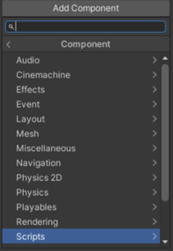
\includegraphics[scale=1]{img/addComponent.png}
	\caption{Añadir un componente a un gameobject}
	\label{fig:componente}
\end{figure}
Algunos de los más componentes predefinidos en Unity más utilizados en el proyecto son los siguientes:
\begin{itemize}
\tightlist
\item \textbf{\textit{Transform}} \cite{doc:Transform}: Este componente lo tienen por defecto todos los gameobjects del juego, y define su tamaño, rotación y posición. Algo a destacar es que los valores de este componente son relativos al contenedor inmediatamente superior del gameObject. Es decir, no es comparable el componente Transform de un gameObject independiente, cuyo contenedor inmediato es la propia escena o el ``mundo'', que el Transform de un gameobject contenido en otro. En este caso su Transform será relativo al gameobject padre.
\item \textbf{\textit{MeshRenderer}}\cite{doc:Transform}:Se encarga de renderizar la malla definida por otro componente llamado \textit{Mesh Filter}, que se encarga de construir una malla desde los assets. Por lo tanto, su función consiste en mostrar las mallas de polígonos en pantalla, teniendo en cuenta el \textit{Transform} del objeto, la luz y otros factores.
\item \textbf{\textit{Collider}}\cite{doc:Collider}: Define el área de colisión de un objeto ante interacciones físicas. Es invisible, y normalmente se utiliza un collider con una forma genérica, como un cubo o una esfera, para aproximarse al volumen del objeto, sin que tenga que ser exacto, para así mejorar el rendimiento general del juego.
Un collider especial es el \textbf{\textit{MeshCollider}}, el cual sí se intenta adaptar lo máximo posible a la geometría original del objeto al que está ligado. Por ejemplo, si el suelo no es plano sino que tiene irregularidades, valles y resaltos, como es el caso, es importante que el collider se adapte bien a su forma para que en todo momento el jugador se pueda apoyar fielmente sobre su superficie.

Además, los colliders pueden tener su propiedad \textit{IsTrigger} marcada, lo que hará que deje de registrar colisiones físicas, y en su lugar se convierta en un ``disparador'' que mandará una señal cuando otro objeto entre o salga de su área de actuación para así poder controlar las acciones que se le indiquen a través de scripts.
\item \textbf{\textit{Rigidbody}}\cite{doc:Rigidbody}: Este componente hace que el movimiento del gameobject sea controlado por físicas, es decir, que pueda ser afectado por la gravedad y otras fuerzas. En conjunción con un collider, el gameobject se verá afectado por las colisiones con otros objetos de manera fiel a como ocurriría en el mundo real.

El jugador, por ejemplo, tiene tanto un rigidbody como un collider, y su movimiento es controlado por fuerzas físicas en lugar de ser desplazado modificando su componente Transform. Esto otorga un mayor realismo de movimiento y de interacción con el entorno

\item \textbf{\textit{AudioSource}}\cite{doc:AudioSource}: Indica que el gameobject puede producir sonidos. Los sonidos emitidos por los gameobjects con este componente pueden ser recogidos por por el componente \textbf{\textit{AudioListener}}. Este debe ser único en la escena y normalmente se encuentra en la cámara principal del juego, al menos en los juegos en primera persona, ya que la cámara actúa como los ojos del jugador, y gracias a este componente, también representaría sus oídos.
\item \textbf{\textit{Animator}}\cite{doc:Animator}: El componente Animator se utiliza para asignar una o varias animaciones a un gameobject. Requiere una referencia a un \textbf{\textit{Animator Controller}}, un  tipo de asset que gestiona el conjunto de clips de animación que puede utilizar, dictando cuándo se debe reproducir cada uno, cómo se mezclan y cómo se transiciona de uno a otro.	
\end{itemize}
\subsection{Prefab}
Un prefab \cite{doc:Prefabs} es un tipo de asset que almacena un gameobject completo, incluyendo sus componentes y propiedades. Actúa como una plantilla reutilizable a partir de la cual se pueden crear nuevas instancias de ese objeto en la escena. De esta manera, si se desea tener varios objetos idénticos, no se tienen que construir todos de cero.\\ Además, si se modifica el prefab, se modificarán automáticamente todas las instancias que existan de él en la escena, lo que resulta muy conveniente a la hora de mejorar o editar varios elementos de forma sencilla y eficiente.
Por ejemplo, este proyecto dispone de un prefab por cada objeto del que se espera más de una copia, como los enemigos, las cajas de suministros, las armas, o los objetos decorativos, entre otros.
\subsection{Shader}
Un shader \cite{doc:Shader} es un conjunto de instrucciones que ejecuta la GPU para definir cómo se deben de renderizar o mostrar los materiales asociados a los objetos.
A partir de un shader se pueden crear varios materiales configurando sus parámetros de textura, color, suavidad, entre otros.

Unity dispone de varios shaders predefinidos disponibles para su uso, como por ejemplo el \textit{Standard Shader}, uno de los más generales y habituales para crear materiales muy variados, o \textit{UniversalRenderPipeline/Lit}, muy utilizado en este proyecto.
Internamente, un shader es un archivo parecido a un script de C\# pero escrito en una combinación de los lenguajes \textit{Cg/HLSL} y \textit{ShaderLab}.
\subsection{Camera}
Una cámara en Unity \cite{doc:Camera} es un objeto que captura y muestra el mundo para mostrárselo al jugador. Cuando se crea una escena, se distribuyen los gameobjects en un espacio tridimensional para crear una composición que el desarrollador quiera conseguir. Una vez colocados, se desea capturar la escena desde una perspectiva determinada para representarla en dos dimensiones, es decir, en imágenes.\\
La cámara se encarga de definir esa proyección de la escena y renderizar los fotogramas en función de lo que capture. El tipo de proyección puede ser ortográfica o con perspectiva. Este último es el elegido para las cámaras del juego ya que, al ser un juego en primera persona, se busca asemejarse a un ojo humano lo máximo posible, y este es el modelo que más se acerca, ya que genera un efecto de profundidad convincente. En el proyecto, la cámara principal seguirá al jugador allá donde vaya y renderizará la vista del jugador.

Se pueden ajustar distintos parámetros de la cámara, como el campo de visión (FOV), utilizado para hacer zoom en algunas armas, o las capas (\textit{layers}) que debe renderizar la cámara. También se pueden aplicar distintos ajustes gráficos como activar el modo HDR para mostrar un mayor rango dinámico, el filtro de suavizado espacial (\textit{antialiasing}) para evitar artefactos en bajas resoluciones, o definir si la cámara permite representar efectos de postprocesado o no.
\subsection{ScriptableObject}
Un scriptableObject \cite{doc:ScriptableObject} es un contenedor de datos que tiene la peculiaridad de ser independiente de las instancias de las clases, es decir, que está definido a nivel de proyecto como un asset más. Es muy útil para almacenar los datos que no van a cambiar en un prefab, ya que cada copia del prefab podrá acceder a los datos del scriptableObject en lugar de tener su propia copia de los datos, lo que permite reducir la carga de memoria de la aplicación.
Su uso en el proyecto se detalla en profundidad en el anexo C.
\subsection{Scripting} \label{Scripting}
El scripting consiste en la creación de scripts dentro del proyecto.Los scripts \cite{doc:Scripts} son archivos que representan una clase dentro de la jerarquía de programación del proyecto, y funcionan como un componente más que se puede ligar a un gameobject. Con ellos, se trata de responder a la interacción del usuario, comunicarse con otros gameobjects, realizar ciertas acciones en función de eventos o modificar sus propiedades en tiempo de ejecución. Cuando se crea un script se define la clase, y cuando se utiliza como componente en algún gameobject, se está creando una instancia de dicha clase.

Los scripts permiten que el juego ``cobre vida'', sea dinámico, interactivo y le dan control al desarrollador para crear los elementos y comportamientos que desee en la aplicación.

El lenguaje utilizado para crear los scripts del juego es C\# \cite{doc:CSharpUnity}, que, en Unity, trabaja con un modelo orientado a objetos y que además es un ``lenguaje administrado'', es decir, que administra la memoria automáticamente.
Cabe mencionar que recientemente en Unity también se puede aplicar un diseño orientado a los datos mediante la nueva pila de tecnología basada en datos (DOTS) multiproceso, pero esta metodología no se aplica en el proyecto.
\subsection{Monobehaviour} \label{Monobehaviour}
Monobehaviour \cite{doc:MonoBehaviour} es la clase base de la que se derivan la mayoría de los scripts vinculados a los GameObjects. Contiene una serie de métodos especiales que son esenciales durante la ejecución del videojuego:
\begin{itemize}
\tightlist
\item \underline{\textit{Awake y Start}}: Estos métodos son similares, ya que ambos son llamados al inicio de la ejecución de un script. Sin embargo, hay algunas diferencias importantes entre ellos:
    \begin{itemize}
    \tightlist
    \item \textbf{\textit{Awake()}} \cite{doc:Awake}: Este método se ejecuta una única vez en el instante en que el script se inicializa en un GameObject. Su ejecución se produce siempre, independientemente de si el gameobject que lo contiene está activo o no: ``activo'' significa que el atributo enabled de la clase \textit{Monobehaviour} tiene un valor verdadero, y por tanto su comportamiento será el definido por sus componentes. En cambio, si el valor de este atributo es falso, el objeto estará ``inactivo'' y no tendrá ningún tipo de comportamiento o actividad asociado. Este método suele utilizarse para inicializar las variables o estados de la clase.
    \item \textbf{\textit{Start()}} \cite{doc:Start}: Este método también es llamado una única vez, pero, a diferencia de \textit{Awake()}, no garantiza que se le llame justo al inicio de la instanciación del objeto en caso de que el objeto, y por tanto el script, no esté activo al momento de la inicialización. Es decir, su ejecución se producirá cuando el gameobject se active, y justo antes de ejecutar por primera vez el método \textit{Update()}, explicado a continuación. Este método resulta muy conveniente cuando un script requiere de otro script para inicializarse. Este último deberá inicializar sus variables en el método \textit{Awake()}, y así estar listo para que el primero lo pueda utilizar, esta vez, en el método \textit{Start()}.
    \end{itemize}
\item \underline{\textit{Update, FixedUpdate y LateUpdate}}: Estos métodos son esenciales en un videojuego, ya que se ejecutarán de forma continuada en forma de intervalos durante la vida de un gameobject. Sin embargo, hay algunas diferencias entre ellos:
    \begin{itemize}
    \tightlist
    \item \textbf{\textit{Update()}} \cite{doc:Update}: Este es el métdodo más común de cualquier script del juego, ya que cualquier elemento que necesite ser actualizado constantemente debe implementarlo.
    
    Es llamado en cada \textit{frame} del juego, es decir, actualiza los elementos deseados justo antes de que se muestren en la pantalla. Sin embargo, hay que tener en cuenta que este método no se ejecuta en intervalos regulares de tiempo, ya que, al ir asociado a los \textit{frames} del videojuego, si un ordenador ejecuta la aplicación a 60 fps (frames por segundo) y otro a 30 fps, el método es llamado 60 y 30 veces respectivamente en 1 segundo. Además, los frames por segundo tampoco son constantes y puede haber unos que requieran más tiempo para mostrarse que otros.
    
    Por lo tanto, se utilizará para comprobar aspectos que no requieran una actualización exactamente precisa. Por ejemplo, el input del usuario o el movimiento de objetos sin propiedades físicas son aspectos que suelen comprobarse en este método.
    \item \textbf{\textit{FixedUpdate()}} \cite{doc:FixedUpdate}: Este método, por su parte, no se relaciona con los frames de la aplicación, sino que es llamado en intervalos regulares de tiempo, ya que tiene la frecuencia del sistema de físicas. Siempre habrá el mismo período de llamadas a este método (concretamente, por defecto es llamado cada 0,02 s). Se suele utilizar para el cálculo de aspectos físicos, y por lo tanto, todo objeto que sea afectado por un Rigidbody debería ser comprobado en este método. Por ejemplo, para calcular trayectorias o bien a la hora de aplicar fuerzas físicas sobre un objeto.
    
    De esta manera se evita tener inconsistencias visuales como saltos o temblores, y asegurar la fluidez de movimiento de los objetos físicos.
    \item \textbf{\textit{LateUpdate()}} \cite{doc:LateUpdate}: Este método es similar al método \textit{Update()}, ya que ese ejecuta antes de cada frame, pero siempre después de que se haya ejecutado el método \textit{Update()}. Resulta útil para establecer un orden de ejecución en elementos que requieran que otros se hayan actualizado antes, por ejemplo, cuando la cámara debe seguir al jugador. La posición del jugador se actualiza en \textit{Update()} y después la cámara actualiza su posición en \textit{LateUpdate()}.
    \end{itemize}
\end{itemize}
El diagrama de la figura \ref{fig:ordenEjecucion} muestra un resumen del orden de ejecución de los métodos principales de un script habitual. También se puede obtener una versión más completa de este \cite{doc:ExecutionOrder}.
\begin{figure}[h]
	\centering
	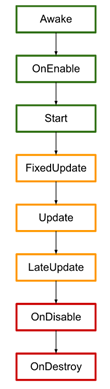
\includegraphics[scale=1]{img/ExecutionOrder.png}
	\caption{Orden de ejecución de los métodos habituales de un script}
	\label{fig:ordenEjecucion}
\end{figure}
\subsection{Modelos 3D}
Un modelo tridimensional de un videojuego se construye mediante una malla (\textit{mesh}). Esta malla está compuesta por vértices (puntos en el espacio) conectados entre sí generando aristas que crean caras poligonales, conformando así la superficie del modelo.

En un motor de videojuegos, los polígonos que forman estas caras son triángulos, ya que es el único polígono que genera un plano en el espacio, independiente de la posición de sus vértices. Cualquier otro polígono podría dar lugar a caras curvadas, lo que generaría errores cuando se rendericen e iluminen dichas caras.

Ello no implica que no se pueda trabajar con otro tipo de polígonos a la hora de modelar los objetos y personajes que se vayan a incluir en el videojuego, como ocurre en otros programas de modelado como Blender. De hecho, suele ser más conveniente utilizar cuadriláteros (\textit{quads}) cuando se crean los modelos del videojuego.
Sin embargo, cuando se importe la malla tridimensional al motor de videojuegos, este convertirá automáticamente todas las caras que la componen en triángulos (este proceso también es conocido como “triangular la malla”) para evitar cualquier tipo de complicación, artefactos inesperados o casos de error complejo cuando se renderiza el modelo.
\subsection{Battle Royale}
El término ``battle royale'' \cite{wiki:BattleRoyale} originalmente proviene de la película japonesa del año 2000 del mismo nombre que presenta un tema similar al de un último jugador en pie.
Más tarde se convertiría en término para referirse a un género específico de videojuegos en el que varios jugadores deben luchar entre ellos hasta que solamente quede un superviviente, que será el ganador de la partida.

Generalmente, una partida comienza distribuyendo de forma aleatoria una gran cantidad de jugadores en un gran mapa, normalmente entre 50 y 100, dependiendo de las dimensiones del mapa.

Se diferencia de los clásicos \textit{shooters} en que incorpora elementos de supervivencia, ya que los jugadores comienzan con un equipamiento nulo y tendrán que encontrar, dispersos por el mapa, cajas, armamento, armaduras, munición y otros elementos beneficiosos para el combate y la supervivencia.\\
Además, el equipamiento de los demás enemigos también puede ser saqueado cuando sean eliminados. Por lo tanto, durante la partida, los jugadores tratarán de equiparse lo mejor posible mientras evitan ser eliminados por otros jugadores.

Un punto clave en este género es que el mapa dispone de una “zona segura” que va disminuyendo su tamaño progresivamente a lo largo de la partida. Esto obliga a los jugadores supervivientes a permanecer en dicha zona, lo que hará que cada vez estén más cerca los unos de los otros y por tanto aumenta las posibilidades de que se encuentren. Los jugadores que se queden fuera de este área irán recibiendo daño incluso hasta ser eliminados si no consiguen entrar en la zona segura rápidamente.

La naturaleza aleatoria de la ubicación de los enemigos y los objetos, así como la reducción del área segura, hacen que el género battle royale sea ideal para desafiar a los jugadores a pensar, actuar rápidamente y mejorar sus estrategias durante el juego para ser el último en pie.
